% Added by Jun Xiong

\section{Models}
We considered four different models to implement our MPS algorithm.
\subsection{AngryBoys Model}
\begin{displaymath}
H = pI + (1-p)\sum_{i=1}^{n-1}\frac{1}{n-1}\sigma_i^x\otimes\sigma_{i+1}^x,
\end{displaymath}
where $I$ is a $2^n\times2^n$ identity matrix and 
\begin{displaymath}
\sigma_i^x = 
\begin{pmatrix}
0 & 1 \\
1 & 0
\end{pmatrix}
\end{displaymath}
As described in 3.1 Model.
The MPO of this model is 
$$
O=W^{[1]}W^{[2]} ... W^{[L]}
$$
And it can be encoded by the operator valued matrices below:
$$
W^{i}=
\begin{pmatrix}
I & 0 & 0 \\
S_x & 0 & 0 \\
0 & qS_x & I
\end{pmatrix}
$$
And  we have $W^1=\begin{pmatrix}p I & q S_x & I\end{pmatrix}$ on the first site of the chain, 
$$W^L=\begin{pmatrix}
I \\ S_x \\ 0
\end{pmatrix}$$
on the last site.

\subsection{RadiatingBoys Model}
\begin{displaymath}
H=p_0 I + p_1 \sum_{i=1}^{n-1}\frac{1}{n-1}\sigma_i^x\otimes\sigma_{i+1}^x + p_2 \sum_{i=1}^{n-2}\frac{1}{n-2}\sigma_i^x\otimes\sigma_{i+2}^x
\end{displaymath}
In this model, the state of a boy could be affected by both its nearest neighbor and its second nearest neighbor. And the MPO can be decomposed into the following matrices:
$$
W^{i}=
\begin{pmatrix}
I & 0 & 0 & 0 \\
S_x & 0 & 0 & 0 \\
0 & I & 0 & 0 \\
0 & p_1 S_x & p_2 S_x & I
\end{pmatrix}
$$
and $W^1=\begin{pmatrix}p_0 I & p_1 S_x & p_2 S_x & I\end{pmatrix}$ and 
$$W^L=
\begin{pmatrix}
I \\ S_x \\ 0 \\0
\end{pmatrix}$$


\subsection{Exponentialboys Model}
\begin{displaymath}
H = P (I + J \sum_{i=1}^{n-1} \sum_{j=i+1}^{n-1} K^{j-i}\sigma_i^x\otimes\sigma_j^x)
\end{displaymath}
The MPO of this model comprises of matrices:
$$W^{i}=
\begin{pmatrix}
I & 0 & 0 \\
S_x & K I & 0 \\
0 & J K S_x & I
\end{pmatrix}
$$,
$W^1=\begin{pmatrix}p_0 I & J K S_x & I\end{pmatrix}$ and 
$$W^L=
\begin{pmatrix}
I \\ S_x \\0
\end{pmatrix}$$.


\subsection{Projectionboys Model}
\begin{displaymath}
H = p_0 I +  \sum_{i=1}^{n-1}(\frac{p_1}{n-1}\sigma_i^x\otimes\sigma_{i+1}^x + \frac{q_1}{n-1}\pi_i^+\otimes\pi_{i+1}^- + \frac{q_2}{n-1}\pi_i^+\otimes\pi_{i+1}^-)
\end{displaymath}
The components of the MPO are:
$$W^{i}=
\begin{pmatrix}
I & 0 & 0 & 0 & 0 \\
S_x & 0 & 0  & 0 & 0 \\
\pi_i^+ & 0 & 0  & 0 & 0 \\
\pi_i^- & 0 & 0  & 0 & 0 \\
0 & p_1 S_x & q_1 \pi_i^+  & q_2 \pi_i^- & I
\end{pmatrix}$$,
$W^1=\begin{pmatrix}p_0 I & p_1 S_x & q_1 \pi_i^+ & q_2 \pi_i^- & I\end{pmatrix}$ and
$$W^L=
\begin{pmatrix}
I \\ S_x \\ \pi_i^+ \\ \pi_i^- \\ 0
\end{pmatrix}$$.

\section{Results}
\subsection{AngryBoys Model}
    Fig.\ref{fig:Angry_result} describes the main data that we obtained through the MPS method. The model here is the Angryboys Model. Fig.\ref{fig:Angry_result}a is the comparison between compressed MPS method and the exact MPS method when the chain size $L=10$ and the bound dimension $\chi=10$. We calculated time evolution of the joint probability, the mean value and the variance, and found that the compressed MPS method agreed well with the exact method. Besides, in this model, all three quantities reach a limit at large enough time, indicating that this model is an aperiodic Markov chain. In Fig.\ref{fig:Angry_result}a, we examined the square error sum of the joint probability between the compressed MPS method and exact method at different bound dimension $\chi$. The figure clearly shows that the error decreases almost exponentially with the increasing bound dimension. And when the bound dimension is close or above 10, the error can be neglected for short chains. This confirms that our approximation is valid. Fig.\ref{fig:Angry_result}c gives the result for a long chain, where $L=100$ and $\chi=10$. Such a long chain case can not be computed by the exact method since the size of the matrix grows exponentially with the chain length. But with our compressed method, we could calculate the physical properties of this long chain in a short time. Here we only used a small bound dimension $\chi=10$ and the size of the matrix is not very large. Thus the MPS method has greatly reduced the computation load in this problem. And the result also reaches a equilibrium state. Fig.\ref{fig:Angry_result}d compares the time evolution of the joint probability of MPS method when the bound dimension $\chi$ is 10 and 20 respectively. At early time, the two bound dimensions will generate slightly different physical quantities, but in the long run, the two cases will converge. Such a converging behavior shows that a bound dimension around 10 can already provide a good approximation on a long chain in Angryboys Model. It indicates that our compressed matrices can simulate the exact result well in the long run, although the matrices have been truncated a lot. However, we need to admit that when the chain size is larger than 200, the code still has some errors and will be interrupted.
    
\begin{figure}[htbp]
\centering
\subfigure[Exact Model(Short Chain)]{
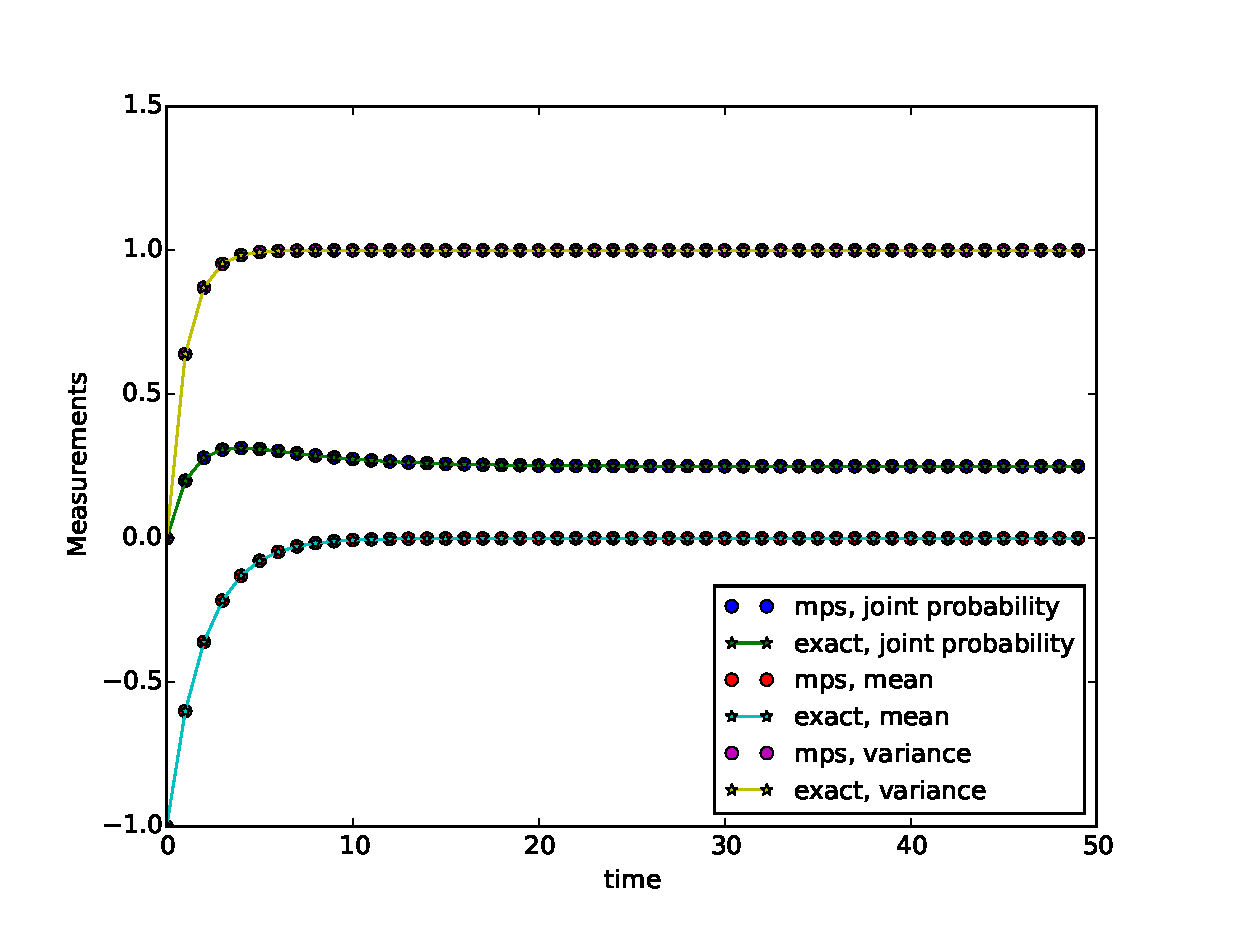
\includegraphics[scale=0.4]{Result_Fig/Angry_Exact_t50_s10_bd10.eps}}\hfill
\subfigure[Error with Different Bound Dimension]{
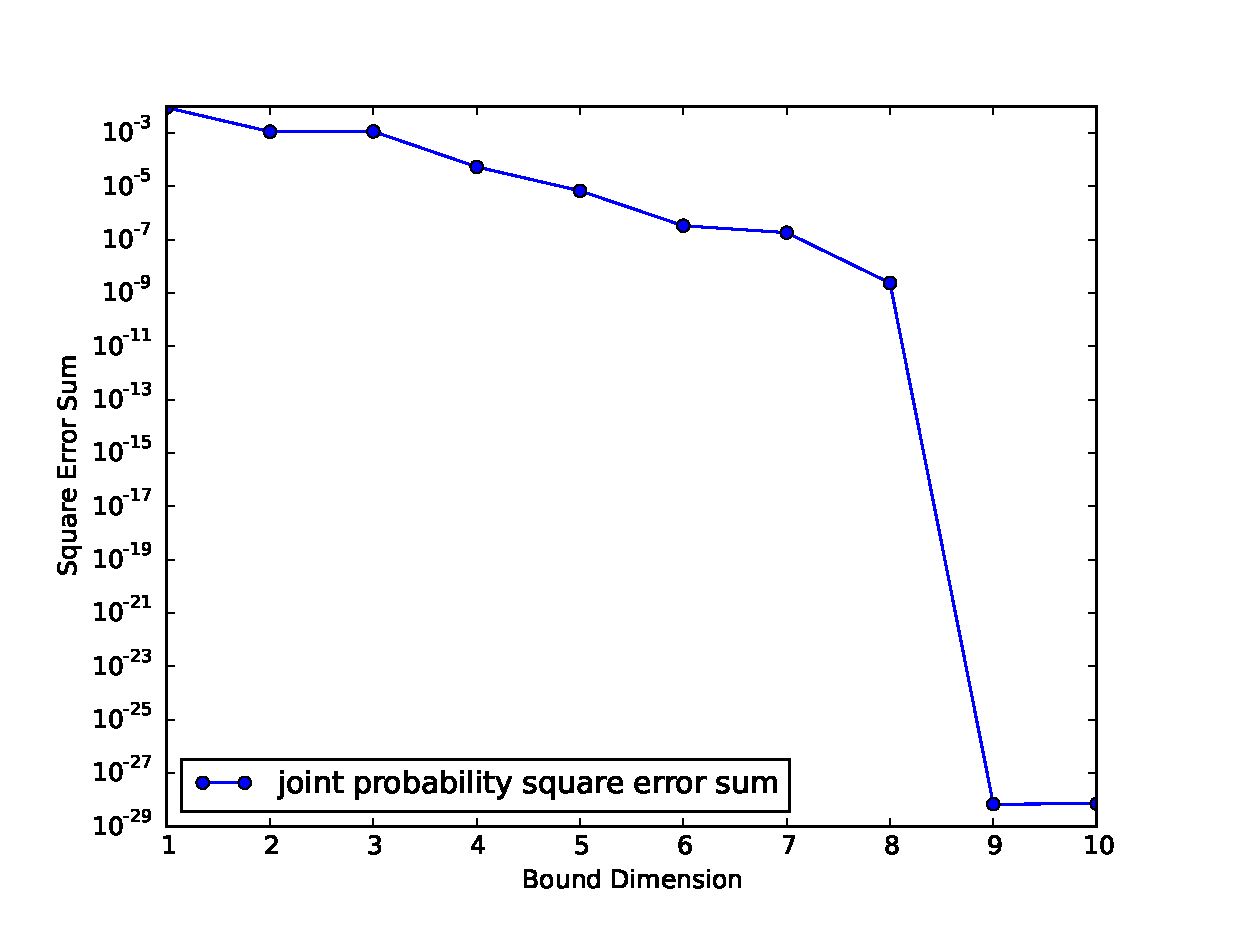
\includegraphics[scale=0.4]{Result_Fig/Angry_Error_t100_s10_bd10_log.eps}}
\subfigure[MPS long chain]{
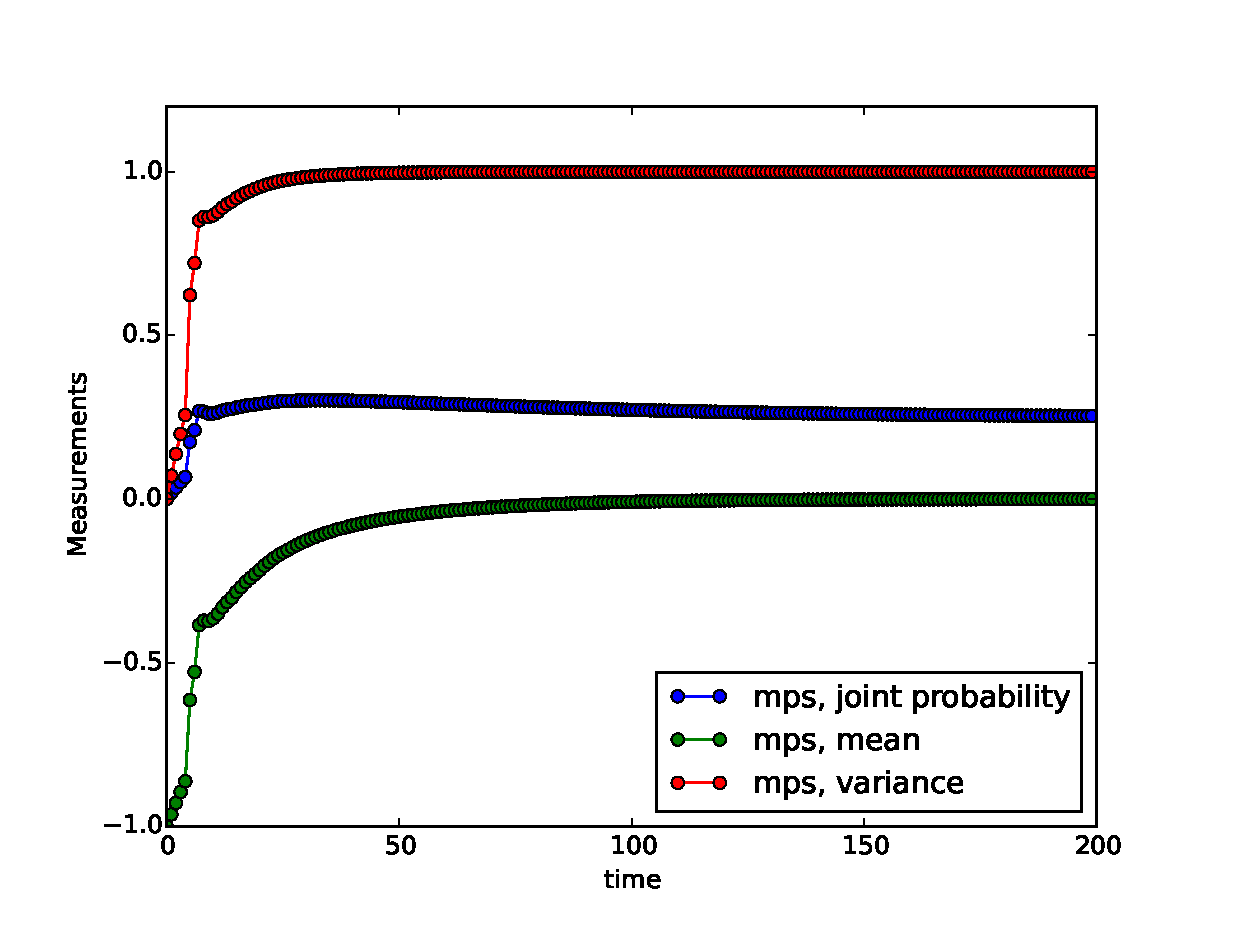
\includegraphics[scale=0.4]{Result_Fig/Angry_MPS_t200_s100_bd10.eps}}\hfill
\subfigure[MPS with Different Bound Dimension]{
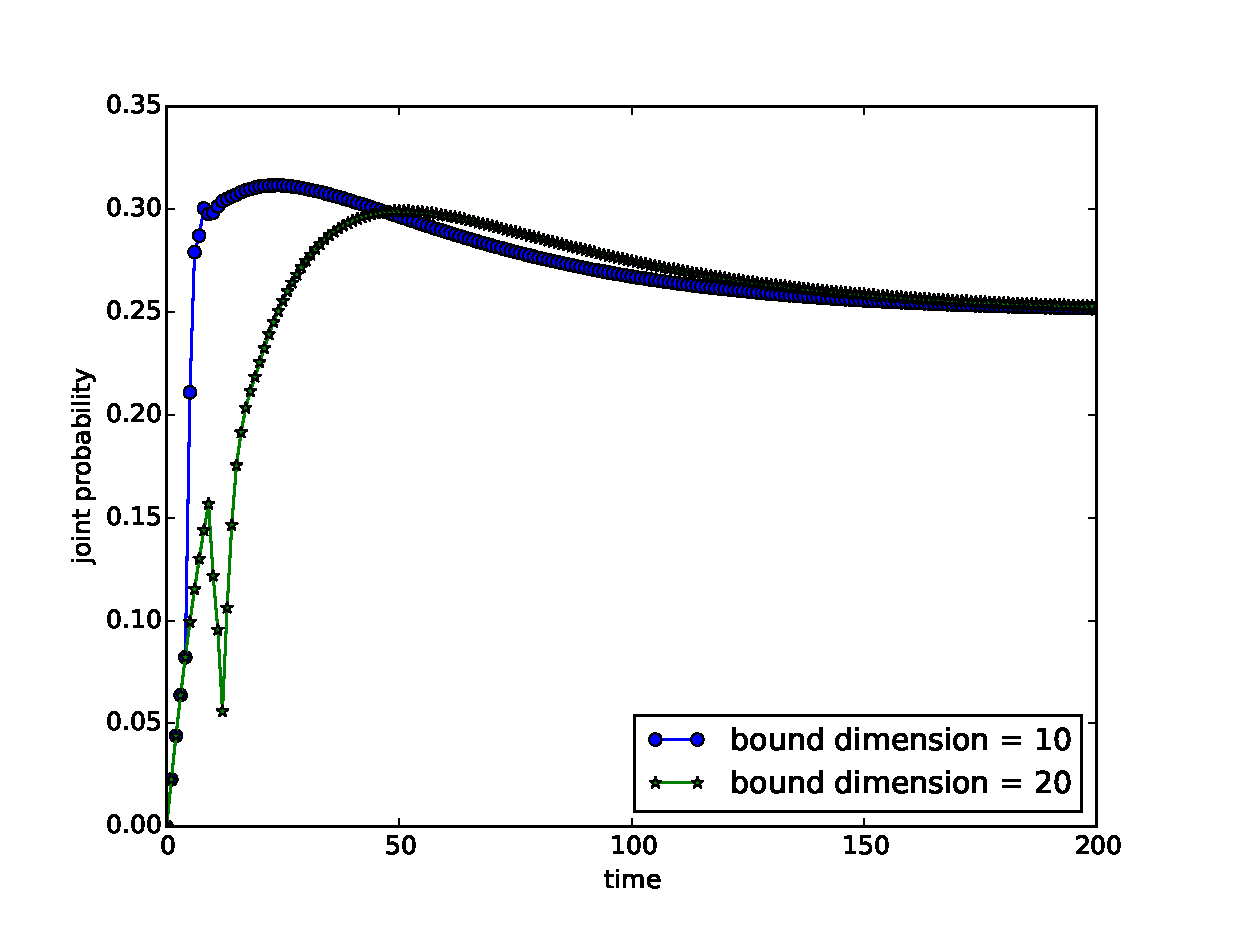
\includegraphics[scale=0.4]{Result_Fig/Angry_MPS_t200_s80_bd10to20.eps}}
  % \end{minipage}\\[1em]
  \caption{Results of Angry Boys Model.(a) gives the comparison of the joint probability, the mean value, and the variance between the MPS method and exact method. The chain size is 10, and the bound dimension $\chi$ is 10 in the MPS method. (b) shows the decay of square error sum with an increasing bound dimensions. The error is computed between the approximation and exact method with a fixed time step of 100. (c) is the result of MPS method on a long chain with the size $L=100$. (d) compares the joint probability of the MPS method with two bound dimensions. The two curves converge in the long run.}
  \label{fig:Angry_result}
\end{figure}

\subsection{RadiatingBoys Model}
Fig.\ref{fig:Radiating_result} is the result of the Radiating Boys Model. 
\begin{figure}[htbp]
\centering
\subfigure[Exact Model(Short Chain)]{
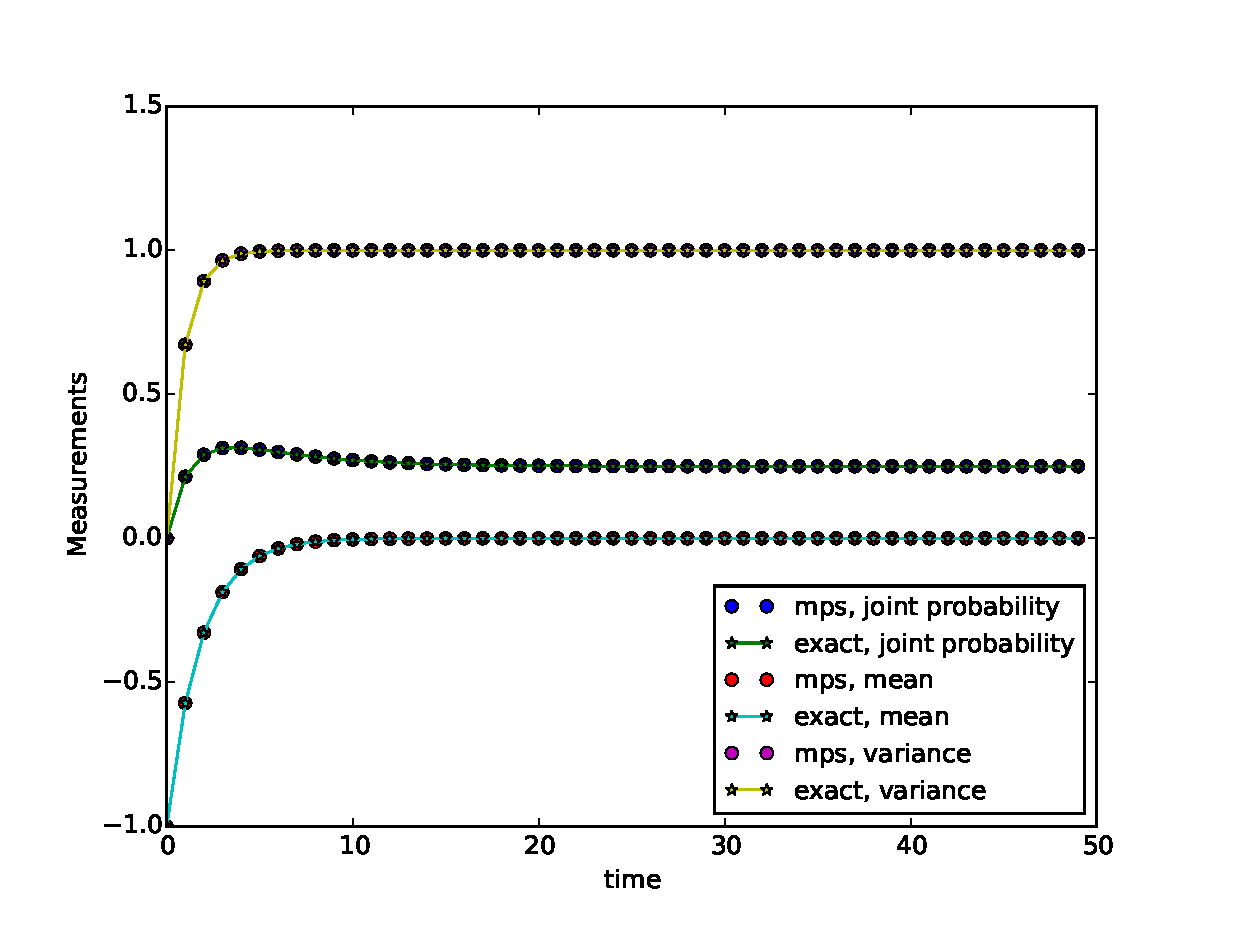
\includegraphics[scale=0.4]{Result_Fig/Radiating_Exact_t50_s10_bd10.eps}}\hfill
\subfigure[Error with Different Bound Dimension]{
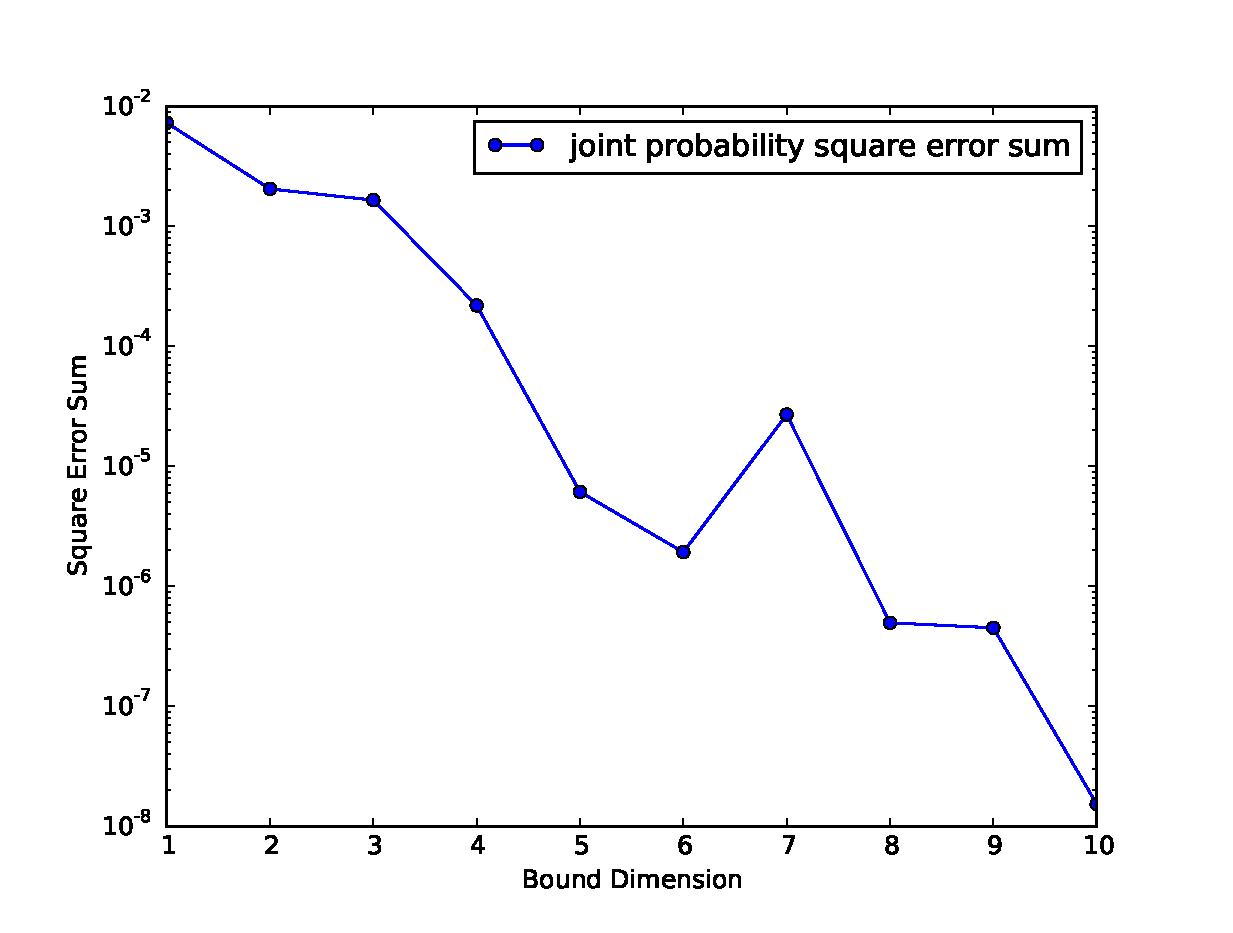
\includegraphics[scale=0.4]{Result_Fig/Radiating_Error_t100_s10_bd10_log.eps}}
\subfigure[MPS long chain]{
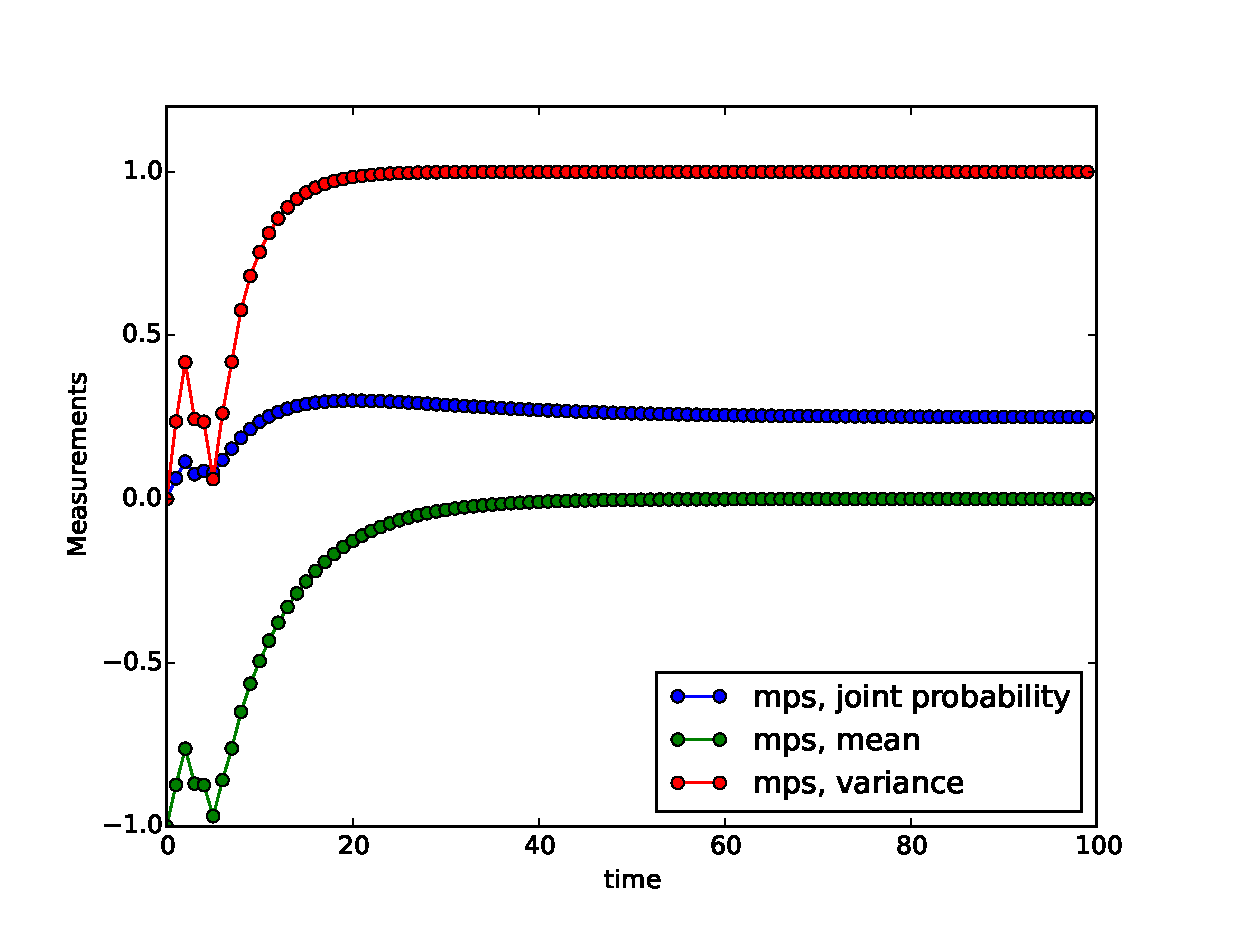
\includegraphics[scale=0.4]{Result_Fig/Radiating_MPS_t100_s30_bd10.eps}}\hfill
\subfigure[MPS with Different Bound Dimension]{
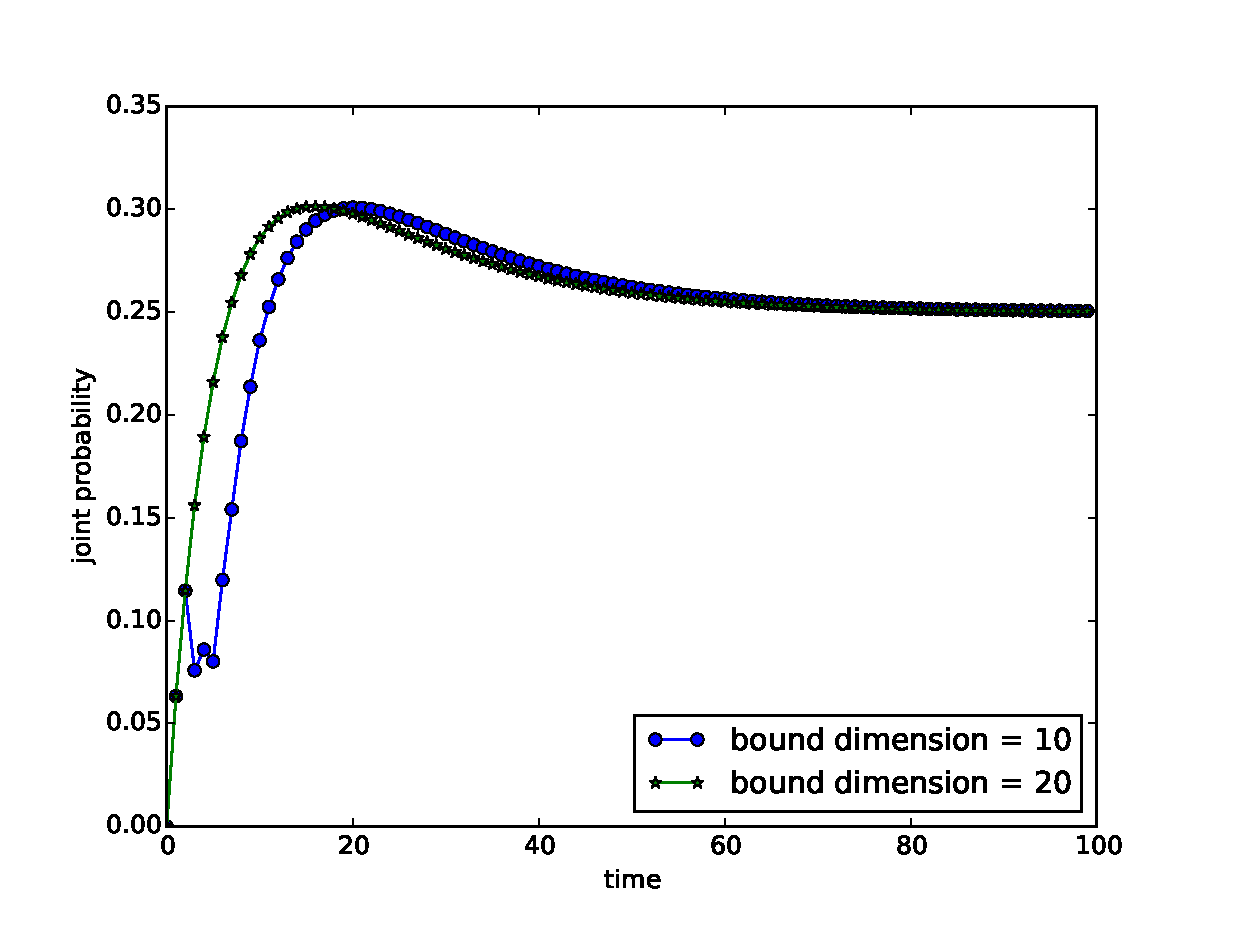
\includegraphics[scale=0.4]{Result_Fig/Radiating_MPS_t100_s30_bd10to20.eps}}
  % \end{minipage}\\[1em]
  \caption{Results of Radiating Boys Model.(a) gives the comparison of the joint probability, the mean value, and the variance between the MPS method and exact method. The chain size is 10, and the bound dimension $\chi$ is 10 in the MPS method. (b) shows the decay of square error sum with an increasing bound dimensions. The error is computed between the approximation and exact method with a fixed time step of 100. (c) is the result of MPS method on a longer chain with the size $L=30$. (d) compares the joint probability of the MPS method with two bound dimensions. The two curves converge in the long run.}
  \label{fig:Radiating_result}
\end{figure}

\subsection{ExponentialBoys Model}
Fig.\ref{fig:Exponential_result} is the result of the Exponential Boys Model. 
\begin{figure}[htbp]
\centering
\subfigure[Exact Model(Short Chain)]{
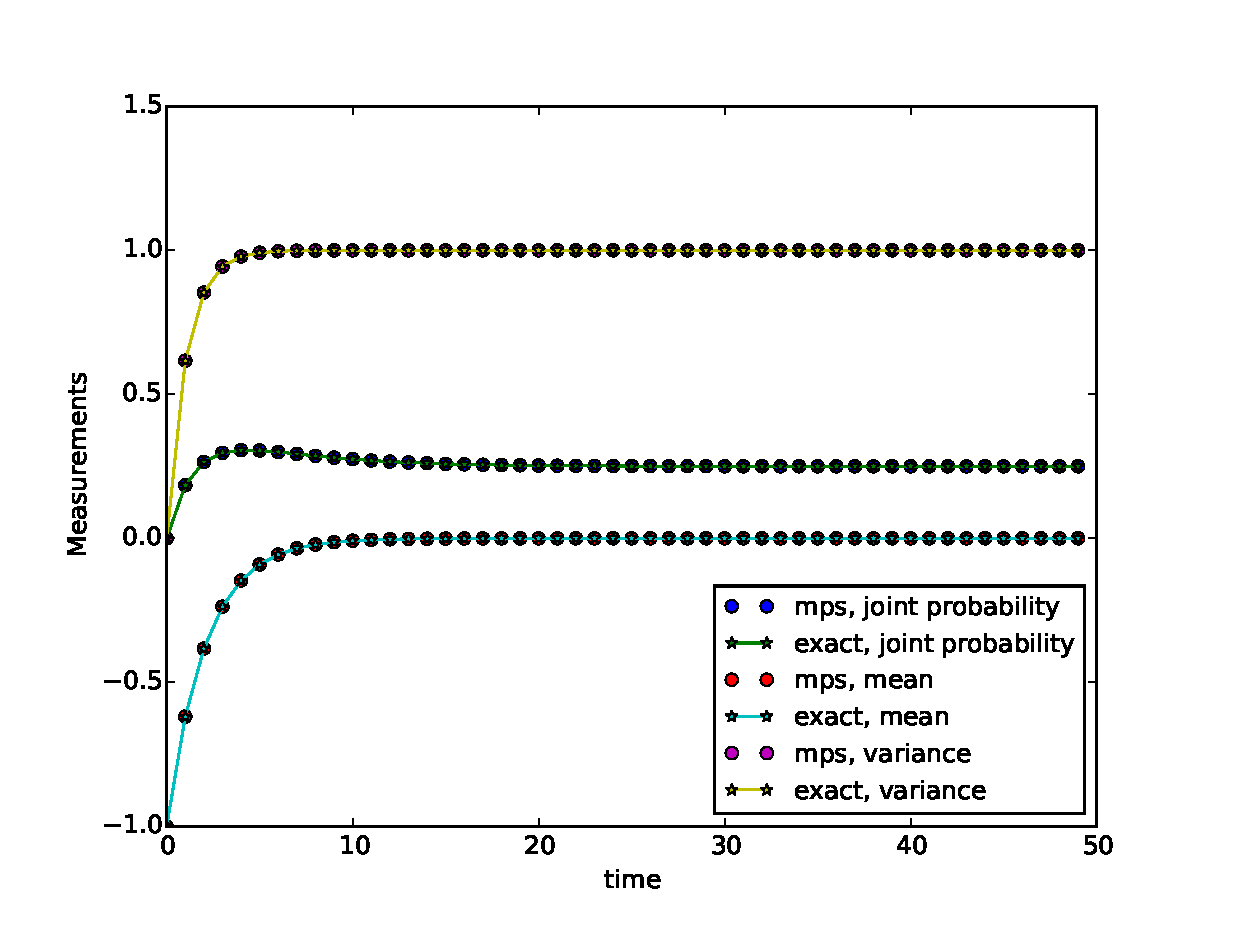
\includegraphics[scale=0.4]{Result_Fig/Exponential_Exact_t50_s10_bd10.eps}}\hfill
\subfigure[Error with Different Bound Dimension]{
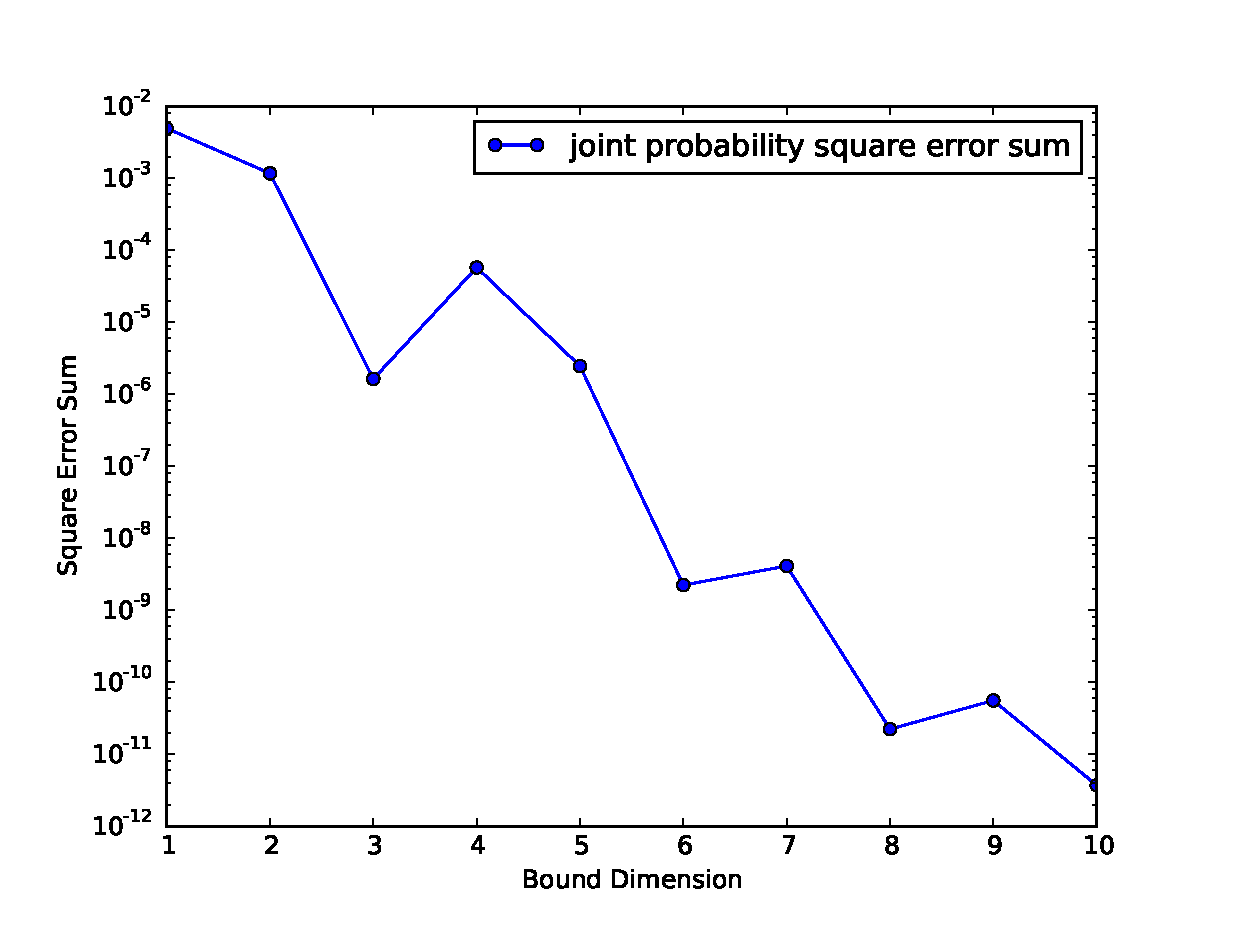
\includegraphics[scale=0.4]{Result_Fig/Exponential_Error_t100_s10_bd10_log.eps}}
\subfigure[MPS long chain]{
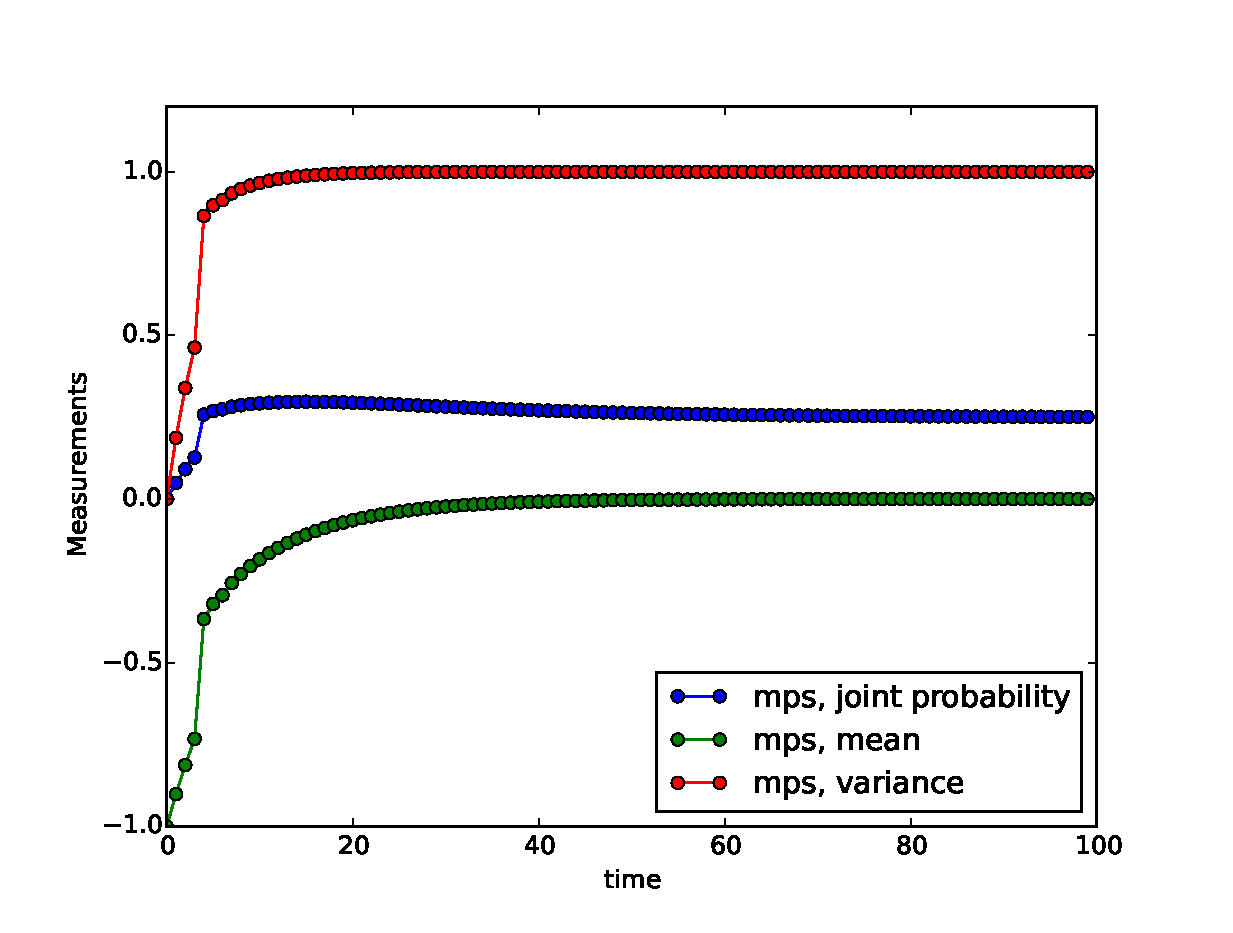
\includegraphics[scale=0.4]{Result_Fig/Exponential_MPS_t100_s40_bd10.eps}}\hfill
\subfigure[MPS with Different Bound Dimension]{
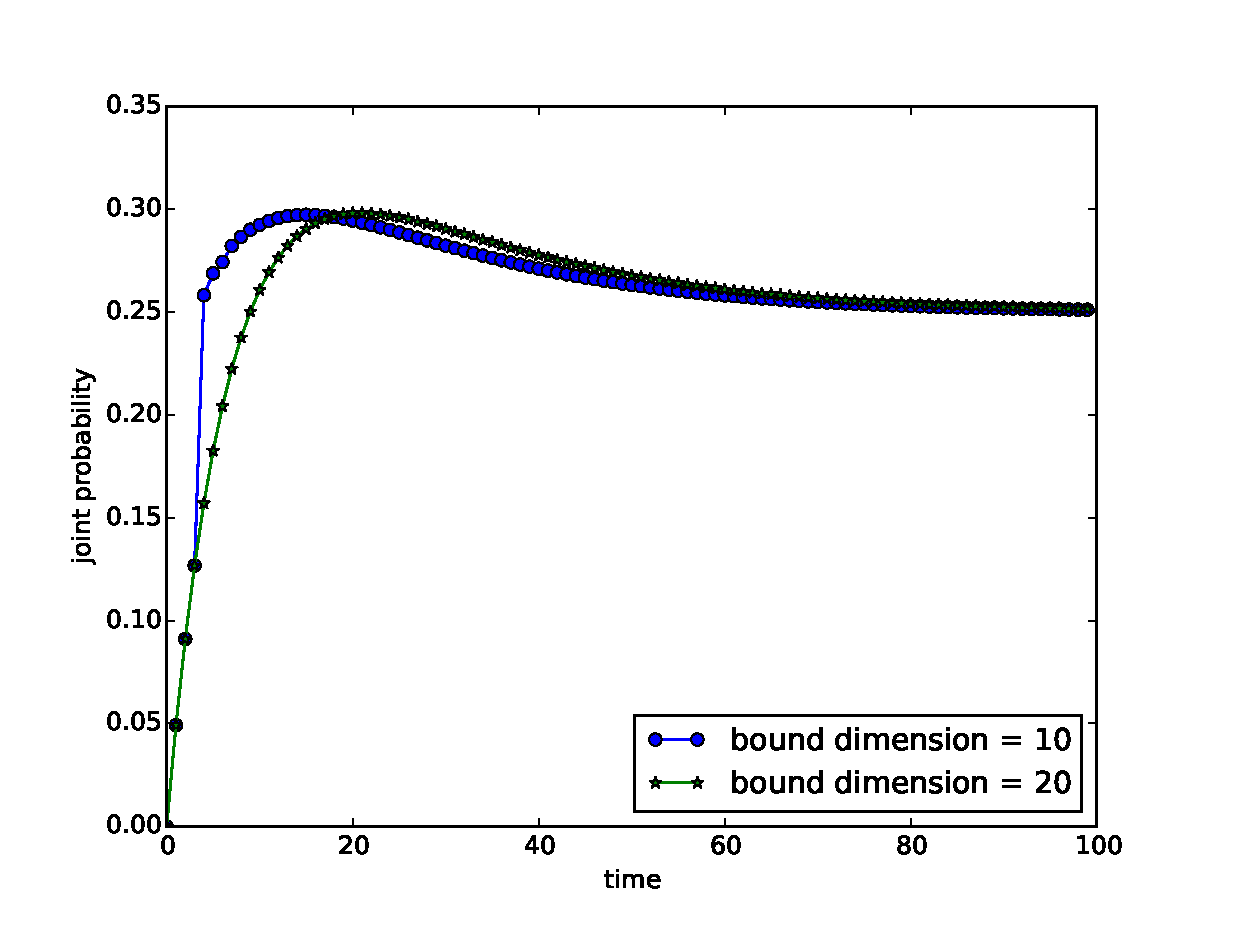
\includegraphics[scale=0.4]{Result_Fig/Exponential_MPS_t100_s40_bd10to20.eps}}
  % \end{minipage}\\[1em]
  \caption{Results of Exponential Boys Model.(a) gives the comparison of the joint probability, the mean value, and the variance between the MPS method and exact method. The chain size is 10, and the bound dimension $\chi$ is 10 in the MPS method. (b) shows the decay of square error sum with an increasing bound dimensions. The error is computed between the approximation and exact method with a fixed time step of 100. (c) is the result of MPS method on a longer chain with the size $L=40$. (d) compares the joint probability of the MPS method with two bound dimensions. The two curves converge in the long run.}
  \label{fig:Exponential_result}
\end{figure}

\subsection{ProjectionBoys Model}
Fig.\ref{fig:Projection_result} is the result of the Projection Boys Model.
\begin{figure}[htbp]
\centering
\subfigure[Exact Model(Short Chain)]{
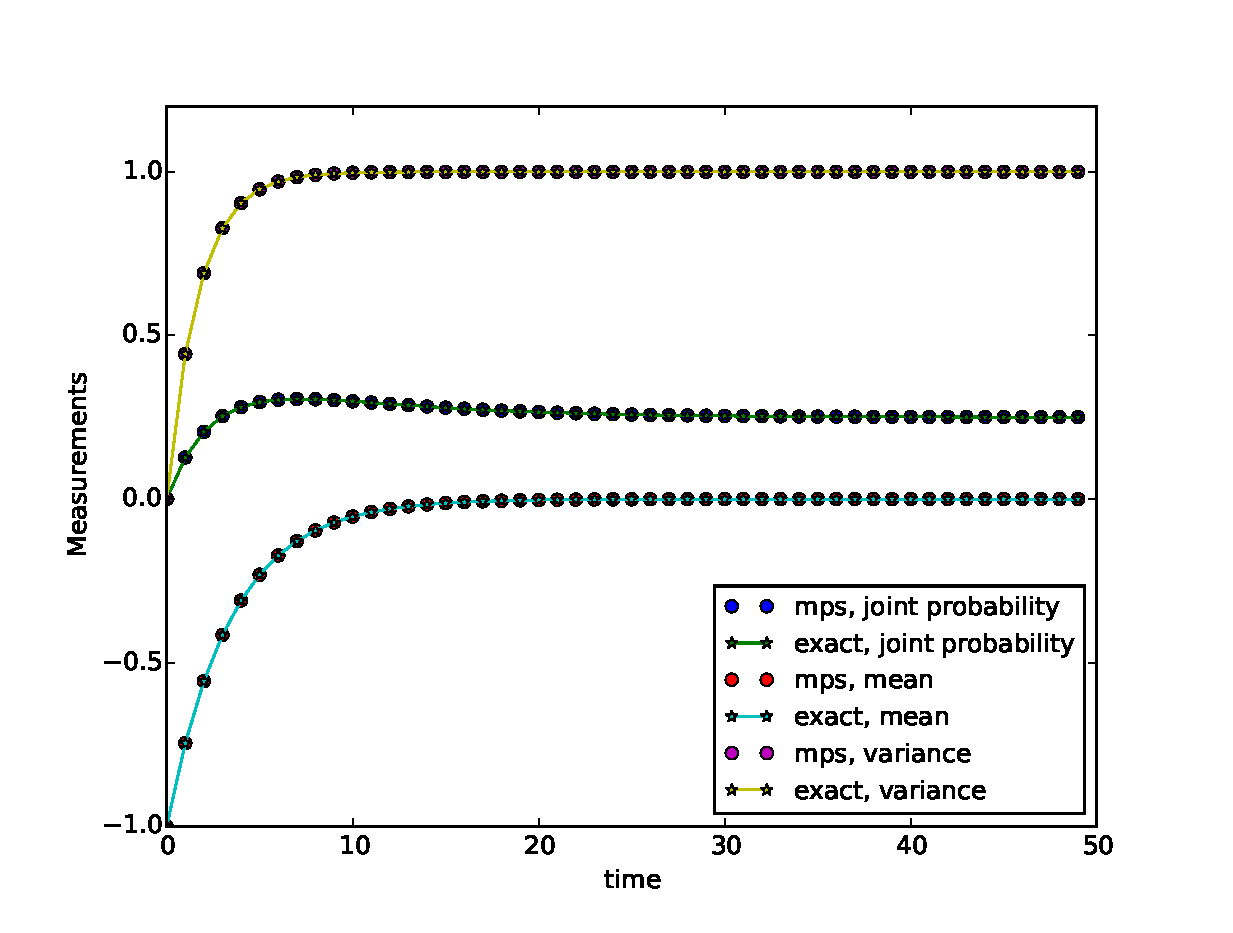
\includegraphics[scale=0.4]{Result_Fig/Projection_Exact_t50_s10_bd10.eps}}\hfill
\subfigure[Error with Different Bound Dimension]{
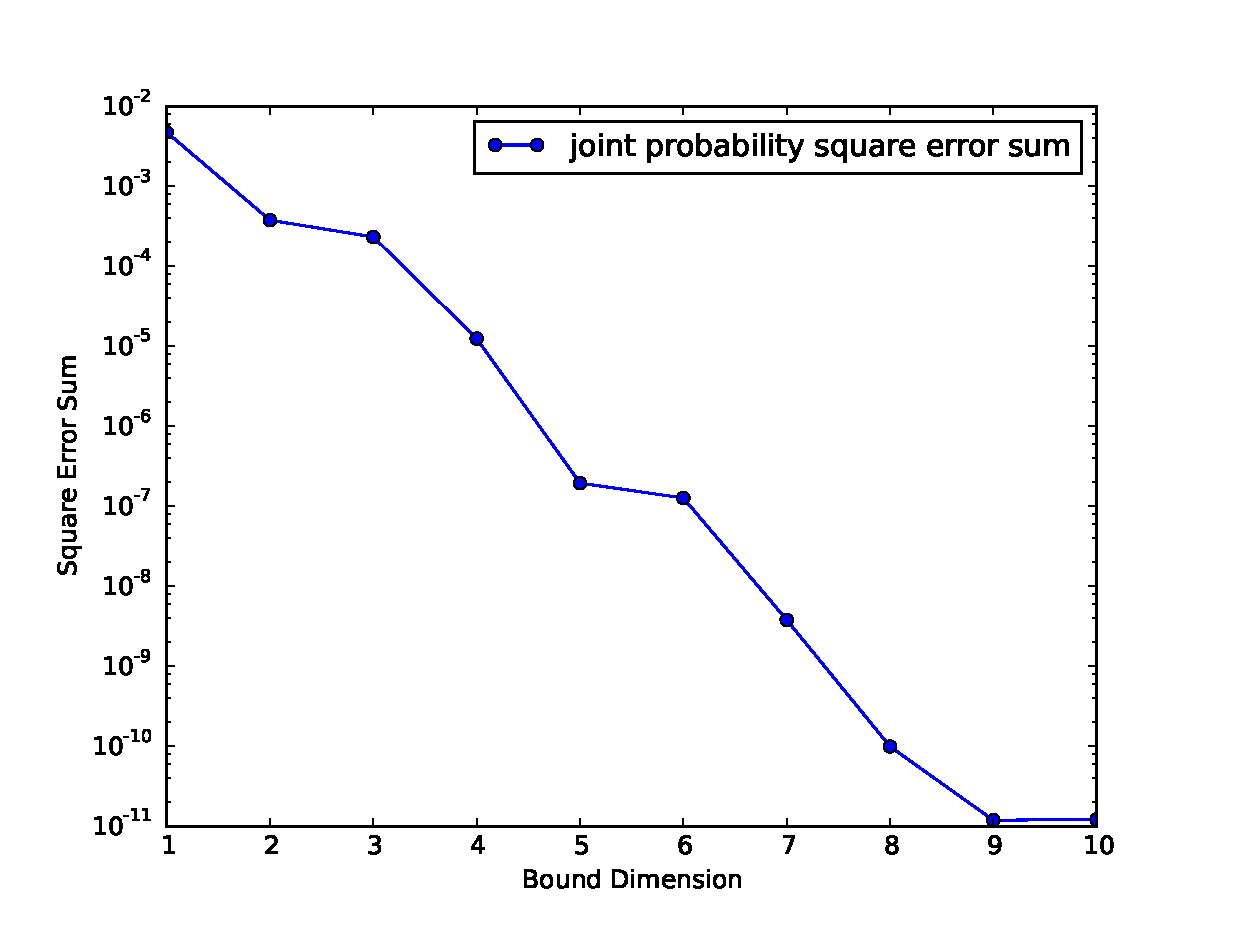
\includegraphics[scale=0.4]{Result_Fig/Projection_Error_t100_s10_bd10_log.eps}}
\subfigure[MPS long chain]{
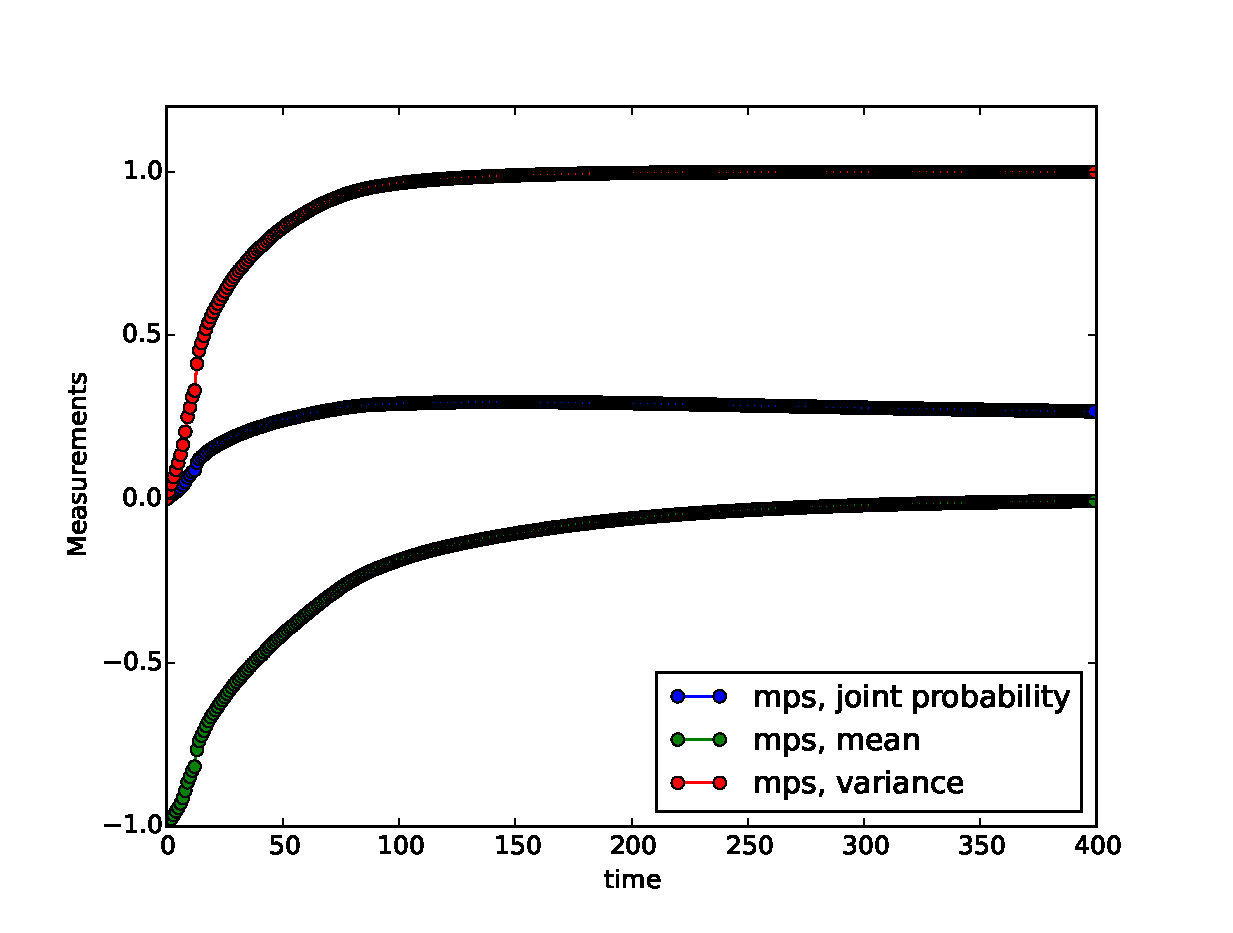
\includegraphics[scale=0.4]{Result_Fig/Projection_MPS_t400_s200_bd10.eps}}\hfill
\subfigure[MPS with Different Bound Dimension]{
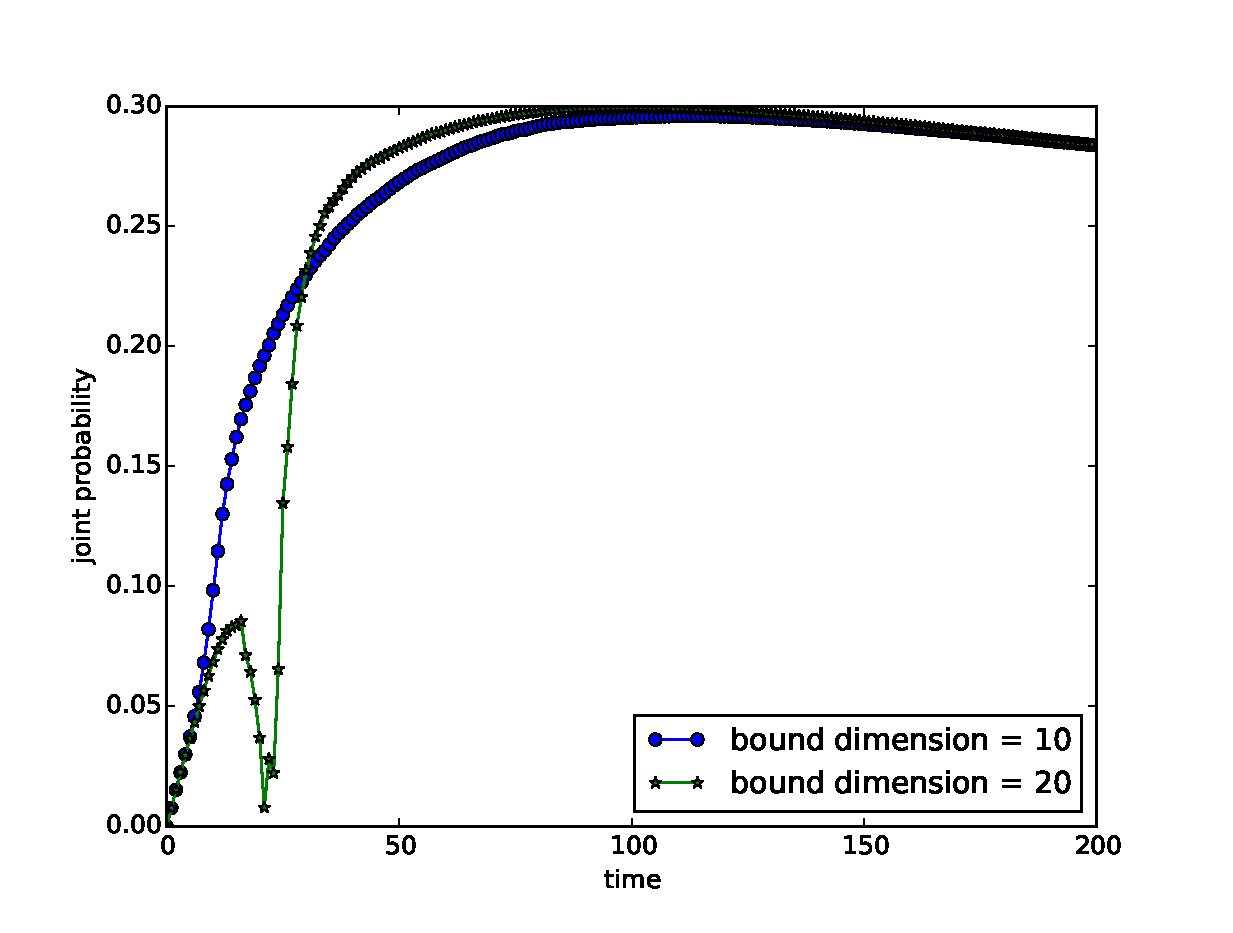
\includegraphics[scale=0.4]{Result_Fig/Projection_MPS_t200_s150_bd10to20.eps}}
  % \end{minipage}\\[1em]
  \caption{Results of Exponential Boys Model.(a) gives the comparison of the joint probability, the mean value, and the variance between the MPS method and exact method. The chain size is 10, and the bound dimension $\chi$ is 10 in the MPS method. (b) shows the decay of square error sum with an increasing bound dimensions. The error is computed between the approximation and exact method with a fixed time step of 100. (c) is the result of MPS method on a long chain with the size $L=150$. (d) compares the joint probability of the MPS method with two bound dimensions. The two curves converge in the long run.}
  \label{fig:Projection_result}
\end{figure}







